\label{chap:evaluation}
Discussed in Chapter \ref{chap:basics}, using the simulated annealing algorithm to find
an optimal memory allocation and the corresponding optimal application profile binding
simultaneously is problematic.
However, a partial success has been achieved.
Given a memory allocation, the simulated annealing algorithm for binding $SA_{\beta}$
yields an good enough profile binding for applications.
This chapter presents the evaluation of $SA_{\beta}$.
The evaluation scenarios are described as following.
$SA_{\beta}$ is implemented according to the design in approach 3 introduced
in Section \ref{subsec:design_3}.
According to this algorithm design,
$SA_{\beta}$ contains the following parameters:
\begin{itemize}
	\item the threshold of the acceptance probability $P_{threshold}$;
	\item the cooling ration $R_{cool}$;
	\item the expected acceptance probability $P_{0}$ at the initial temperature;
	\item factor $F_{iteration}$ that used for computing the maximum number of
	the inner loop iterations
\end{itemize}
In all evaluation scenarios, the parameters are set as following:
\begin{itemize}
	\item $P_{threshold}=0.001$;
	\item $P_{0=0.9}$;
	\item $R_{cool} = 0.9$;
	\item $F_{iteration}=1$
\end{itemize}
The data sets and ILP resutls provided by the authors of \cite{Strobel2016}
are used as the input for $SA_{\beta}$.
The data sets contain the informations of following contents:
\begin{itemize}
	\item A set of 79 memory types;
	\item A set of 4 applications, namely $IP reassembly$, $IP check$, $MD5$, $Huffman$
		  \cite{Strobel2016};
	\item 4 sets of profiles corresponding to the set of applications;
	\item An interconnect.
\end{itemize}
For each application, $SA_{\beta}$ is performed individually on an
$Intel^{\text{\textregistered}} \text{ } Core^{\text{\texttrademark}}2 \text{ }
Quan \text{ } CPU \text{ } Q9300$ system
clock at 2.5 GHz and having 7.7 GB main memory. 
The corresponding optimal memory allocation provided by the ILP result is given
to $SA_{\beta}$.
In Section \ref{sec:evalution_p_1}, the results of $SA_{\beta}$ is compared with
the results provided by ILP.
Section \ref{sec:evalution_p_2} evaluates $SA_{\beta}$ by adjusting the algorithm
parameters.
	\section{Results comparison between $SA_{\beta}$ and ILP}
	\label{sec:evalution_p_1}
	To verify its functionality, $SA_{\beta}$ is performed for all applications.
	ROM and RAM modes are both taken into consideration. Due to the fact that
	$SA_\beta$ is a random searching algorithm, its output may be different
	for each execution. According to this, $SA_{\beta}$ is executed for five times
	for each application. Figure \ref{fig:EVA_ROM} and Figure \ref{fig:EVA_RAM}
	show the results for ROM mode and RAM mode respectively. In the figures, the
	ILP results are provided by the authors of \cite{Strobel2016} and they are
	used as the references for the $SA_{\beta}$ evaluation.
	In the figures, the error percentage is defined by Equation \ref{equa:error},
	where $P_{SA_{\beta}}$ and $P_{ILP}$ are the power costs of the $SA_{\beta}$
	results and ILP results respectively.
	\begin{equation}
	\label{equa:error}
	Error \text{ } percentage = \dfrac{P_{SA_{\beta}}-P_{ILP}}{P_{ILP}}
	\end{equation}
	For the simplification of comparing $SA_{\beta}$ results and ILP results,
	the power cost and the the error percentage are mainly focused.
	If the power costs $P_{SA_{\beta}}$
	obtained by $SA_{\beta}$ is close enough to the power cost $P_{ILP}$
	provided by ILP, the binding output by $SA_{\beta}$ is considered as
	good enough because ILP yields the optimal binding.
	More specifically, the bindings with power error percentage lower
	than 5\% are considered to be near optimal.
	The details of bindings are not shown in the results.
	\begin{figure}[htb]
		\begin{center}
			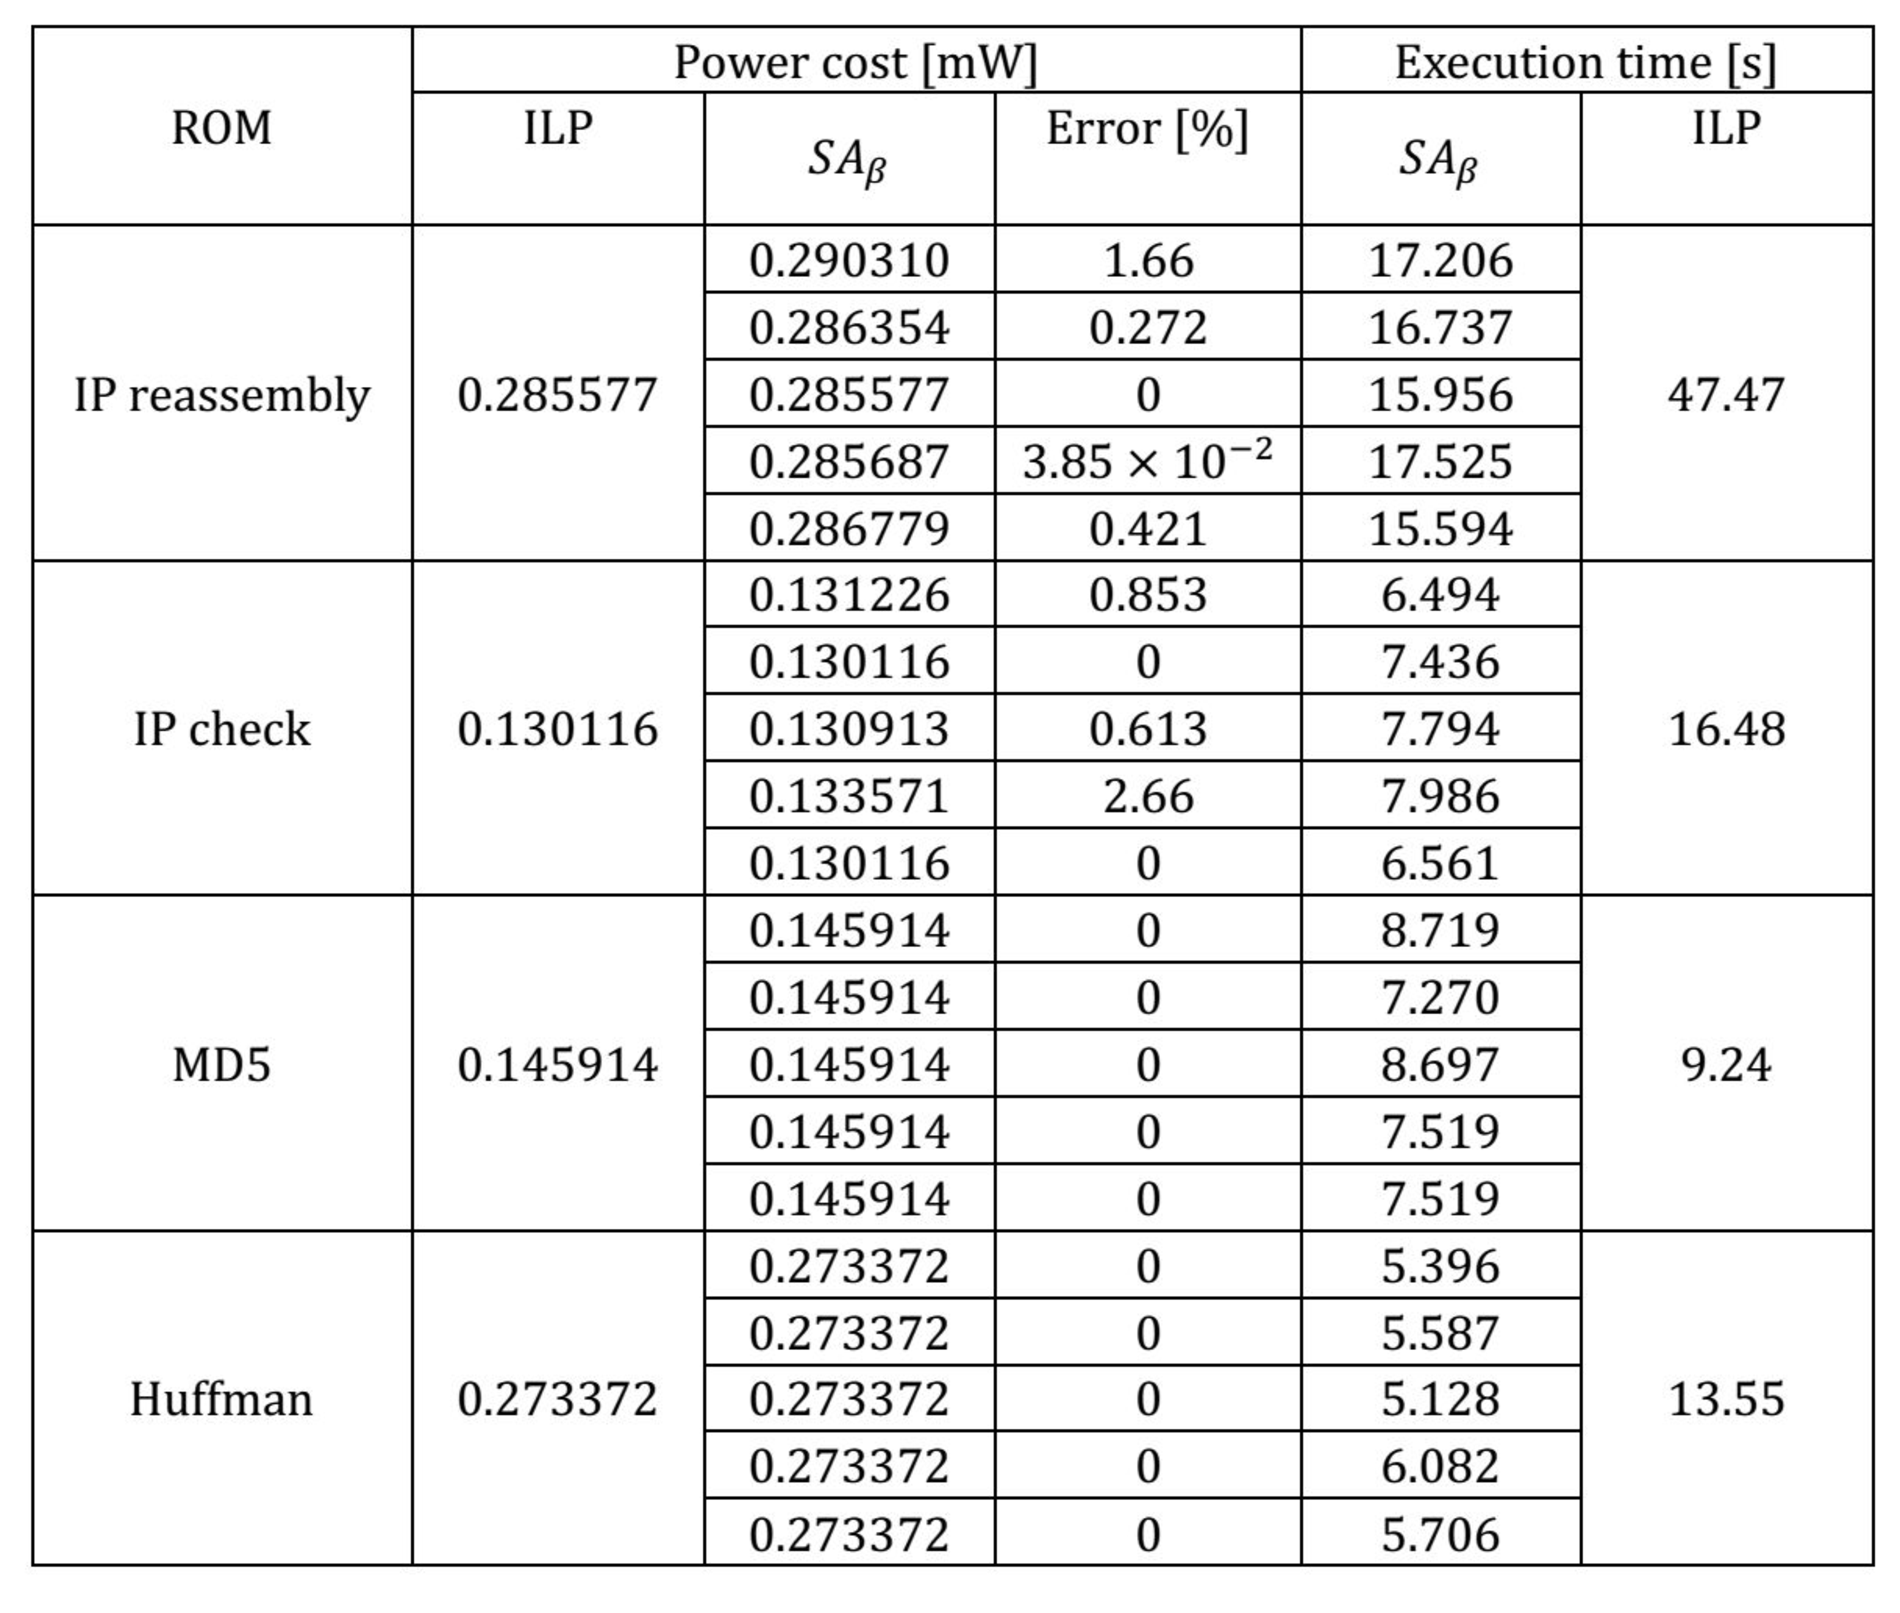
\includegraphics[width=0.7\textwidth]{EVA_ROM}
			\caption{Results Comparison between $SA_{\beta}$ and ILP (ROM)}
			\label{fig:EVA_ROM}
		\end{center}
	\end{figure}
	\begin{figure}[htb]
		\begin{center}
			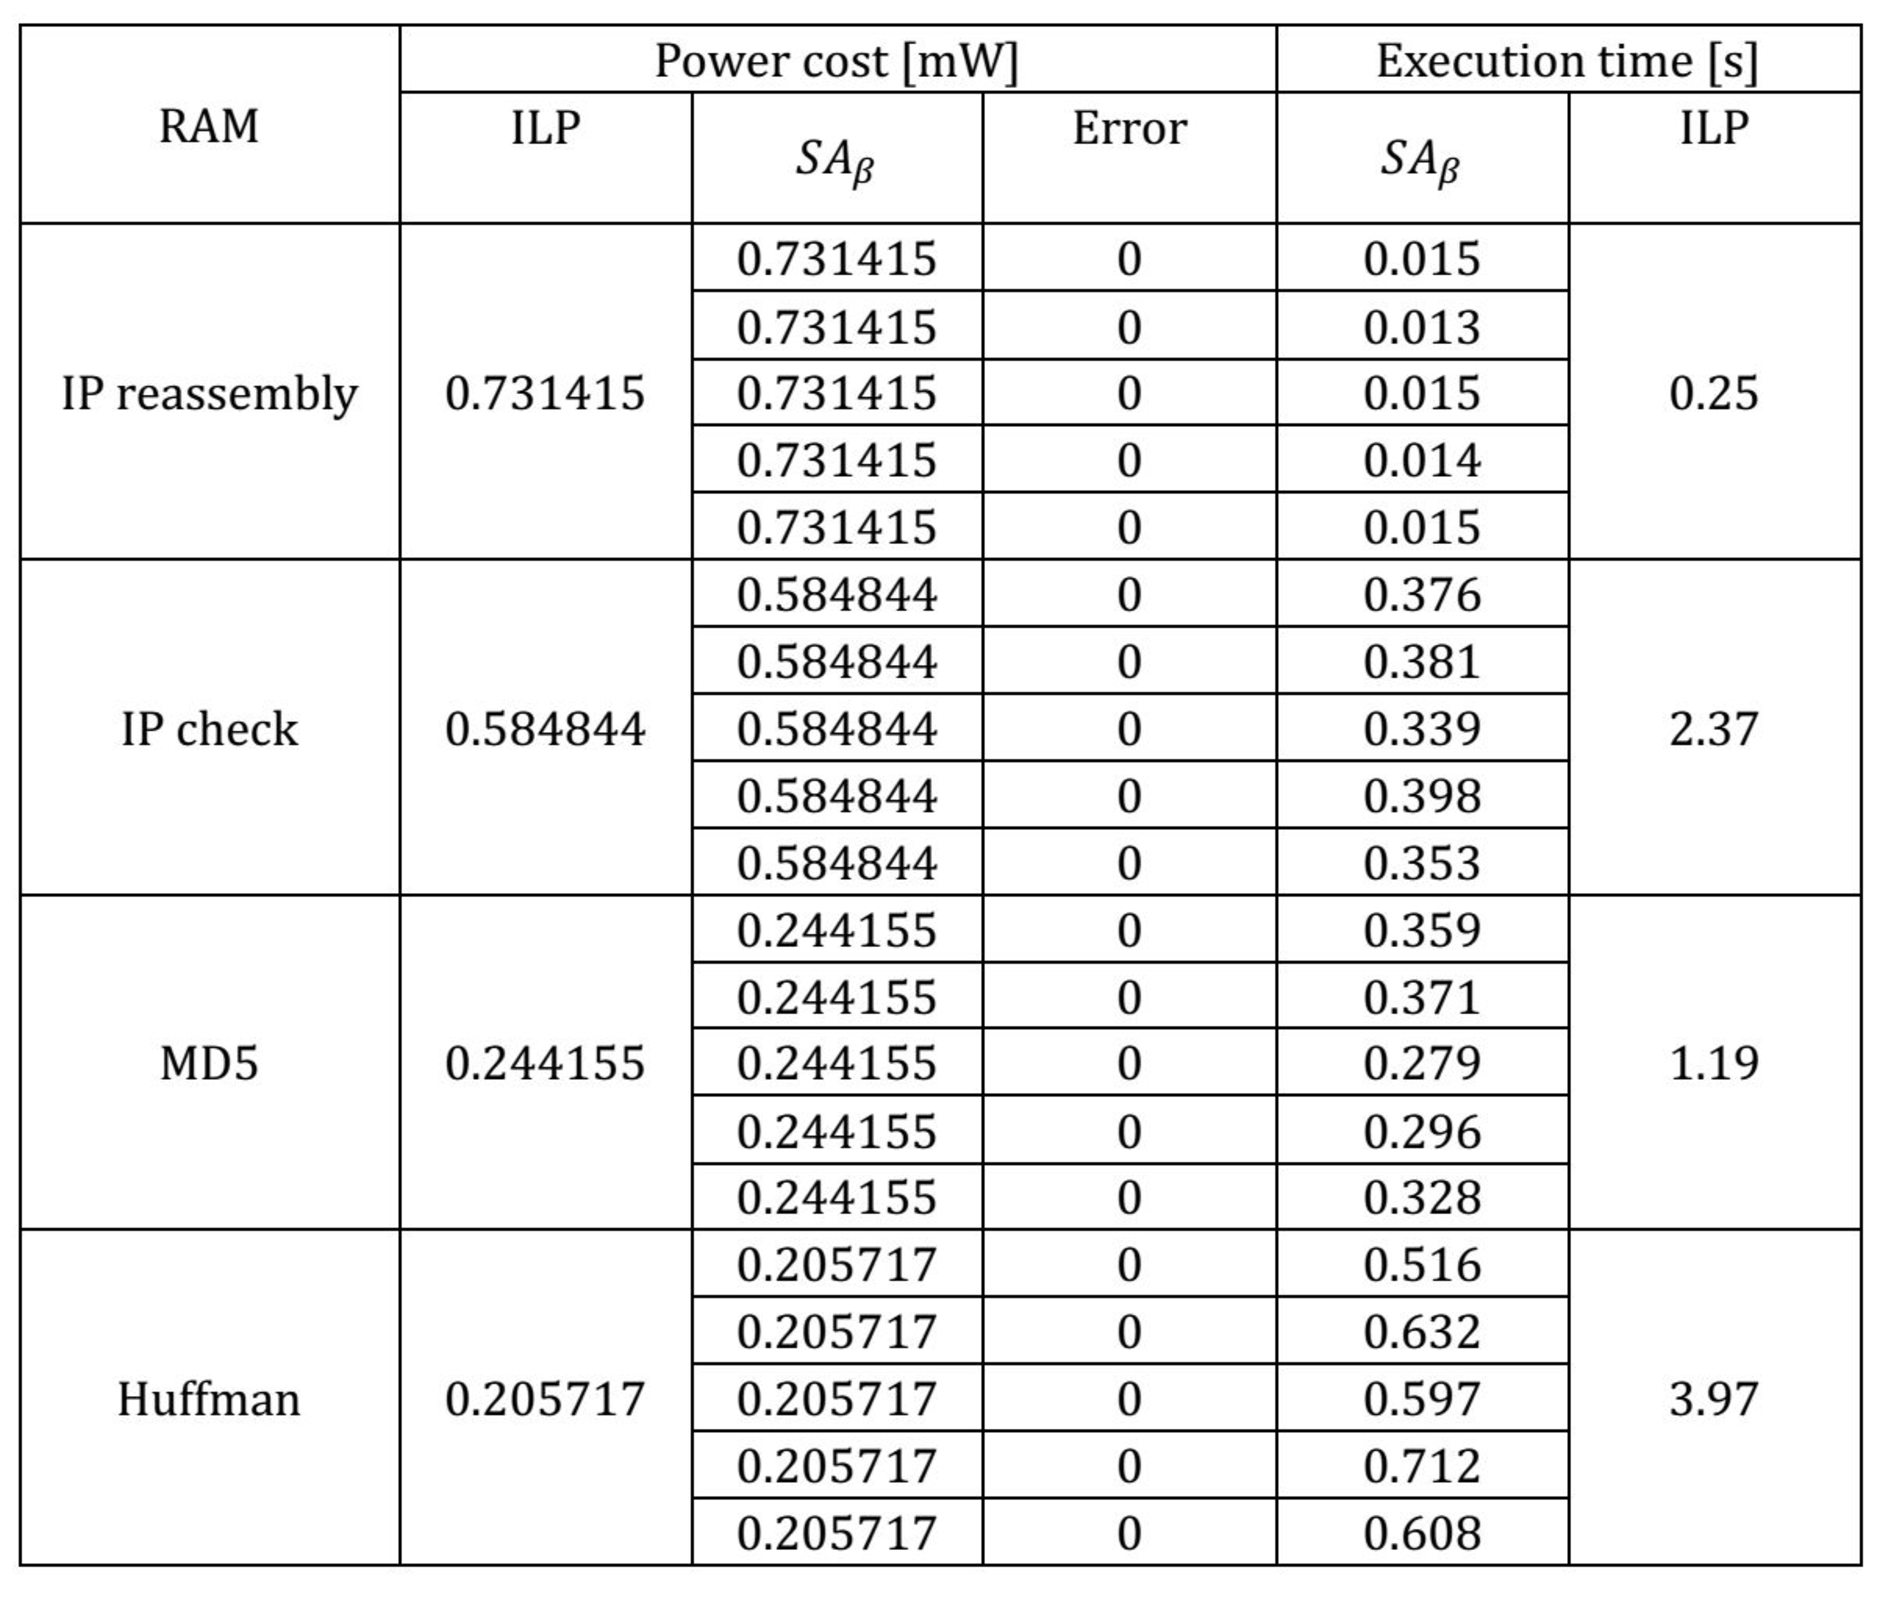
\includegraphics[width=0.7\textwidth]{EVA_RAM}
			\caption{Results Comparison between $SA_{\beta}$ and ILP (RAM)}
			\label{fig:EVA_RAM}
		\end{center}
	\end{figure}

	From the results of ROM mode shown in Figure \ref{fig:EVA_ROM},
	it is can be seen that for application
	MD5 and Huffman, $P_{SA_{\beta}}$ are exactly the same with $P_{ILP}$
	in each execution of $SA_{\beta}$.
	For application IPreassembly anb IPcheck, $P_{SA_{\beta}}$
	is slightly different from $P_{ILP}$ in some executions of $SA_{\beta}$.
	However, the error percentages in such cases are rather small.
	The bindings output by $SA_{\beta}$ in these cases are near optimal.
	From the results of RAM mode shown in Figure \ref{fig:EVA_RAM},
	it is clear that $P_{SA_{\beta}}$ is exactly the same with $P_{ILP}$
	in each execution of $SA_{\beta}$ for all applications. The output
	bindings are optimal. Therefore, the functionality of $SA_{\beta}$
	is verified.
	
	For the execution time, there is no comparability between $SA_{\beta}$
	and ILP because of the pre-condition that the optimal memory allocation is
	given to $SA_{\beta}$. This pro-condition makes the execution time
	of $SA_{\beta}$ shorter than that of ILP for all applications.
	
	\section{Parameters adjustment of $SA_{\beta}$}
	\label{sec:evalution_p_2}
	One important feature of simulated annealing algorithm is the trade-off
	between efficiency and accuracy by adjusting the algorithm parameters.
	To verify this feature, the following testing scenarios are created.
	Application IPreassembly in ROM mode is used for all testing scenarios.
	In each testing scenario, only one parameter is adjusted while the others
	are kept the same with the setting used in Section \ref{sec:evalution_p_1}. 
	For each testing scenario, $SA_{\beta}$ is performed five times.
	The average power error percentage and the average execution are measured.
	The corresponding results are represented in Figure \ref{fig:EVA_P_THRESHOLD} to
	Figure \ref{fig:EVA_FACTOR}.
	
	\begin{figure}[htb]
		\begin{center}
			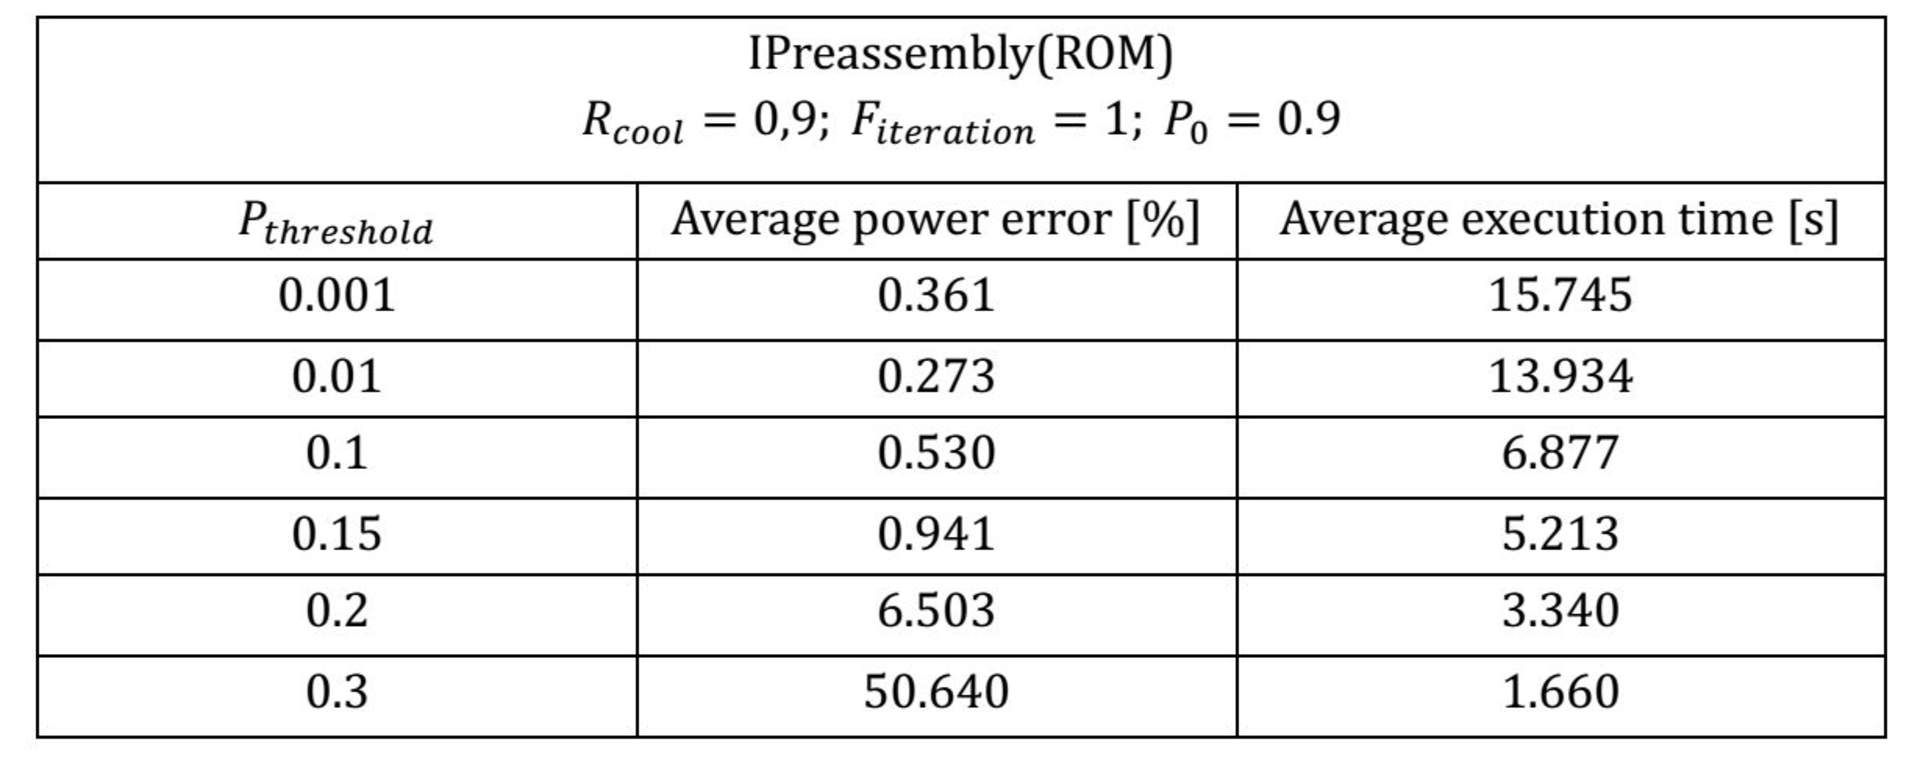
\includegraphics[width=0.7\textwidth]{EVA_P_THRESHOLD}
			\caption{Results of $P_{threshold}$ Adjustment}
			\label{fig:EVA_P_THRESHOLD}
		\end{center}
	\end{figure}

	Figure \ref{fig:EVA_P_THRESHOLD} shows the results of using different value for
	$P_{threshold}$ in $SA_{\beta}$. From the figure it is can be seen that
	if $P_{threshold}$ is increased, the average power percentage increases as well.
	This means that $SA_{\beta}$ terminates too early due to the high $P_{threshold}$.
	The possibility to accept a worser binding is also very high. Thus, $SA_{\beta}$
	may not provide a good enough binding. In the $P_{threshold}$ equals to 0.2,
	the average power error percentage is lager than 5\%. The binding provided by $SA_{\beta}$
	in this case is not near optimal. The result in the case of $P_{threshold}$
	equals to 0.3 is much worser and it is unacceptable.
	
	From Figure \ref{fig:EVA_P_THRESHOLD} it is also can be seen that the average
	execution time decreases with the increase of the average power error percentage.
	This means that by scarifying the accuracy, a better efficiency can be obtained in $SA_{\beta}$.
	It is noticed that in the first 4 cases shown in the figure, the average power error
	percentages are all lower than 1\%. The bindings with such average power error
	percentages are considered as valuable. But the execution times of case $P_{threshold}$
	equals to 0.1 and $P_{threshold}$ equals to 0.15 are much shorter than that of
	the other two. The performance of $SA_{\beta}$ can be improved without losing
	too much accuracy if the $P_{threshold}$ is set in the range of 0.1 to 0.15 for
	this testing scenario.
	
	\begin{figure}[htb]
		\begin{center}
			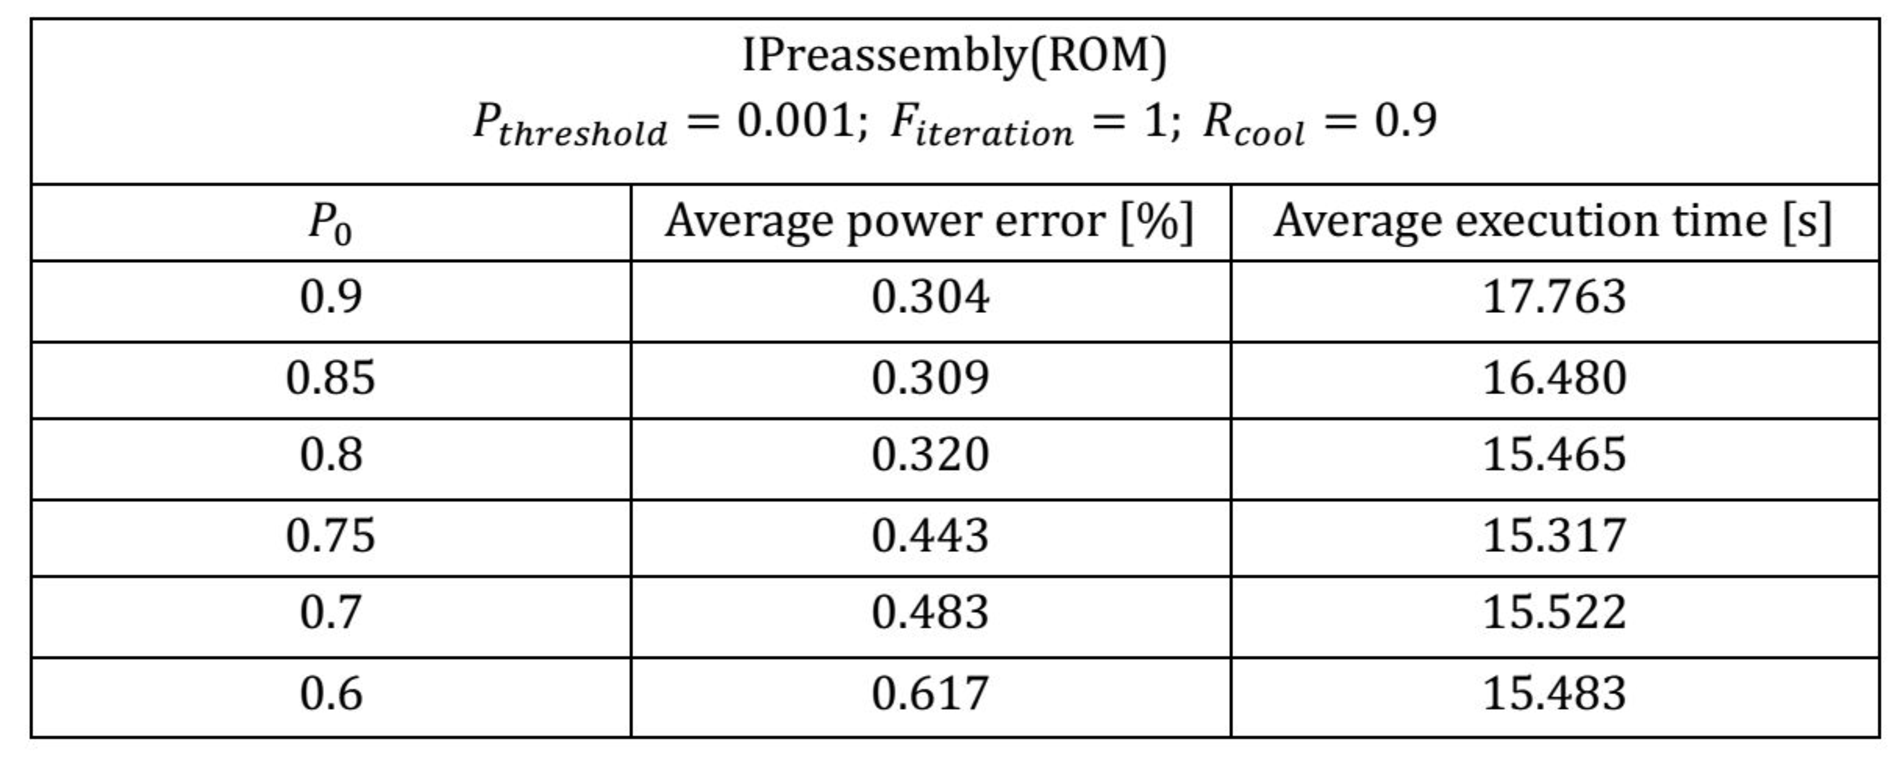
\includegraphics[width=0.7\textwidth]{EVA_P_0}
			\caption{Results of $P_{0}$ Adjustment}
			\label{fig:EVA_P_0}
		\end{center}
	\end{figure}

	Figure \ref{fig:EVA_P_0} shows the results of setting $P_{0}$ to different values.
	From the figure it is can be seen that with the adjustment of $P_{0}$,
	there is no huge change for neither the average power error percentage nor the average
	execution time. The efficiency and accuracy of $SA_{\beta}$ are not affected by the
	value of $P_{0}$.

	

	\begin{figure}[htb]
		\begin{center}
			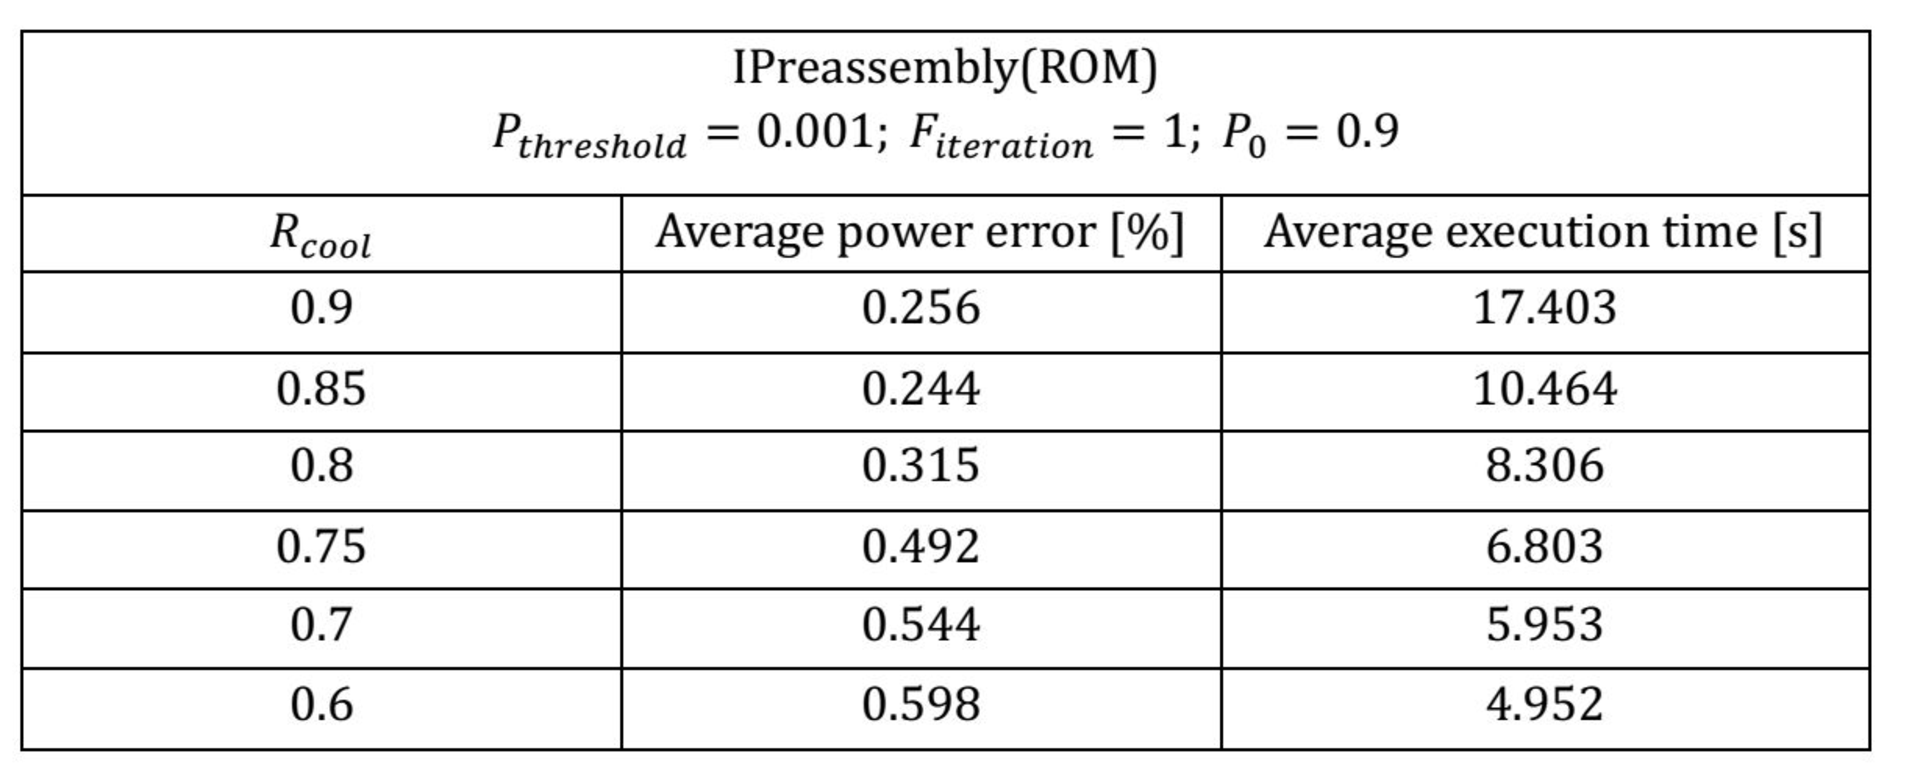
\includegraphics[width=0.7\textwidth]{EVA_COOLING}
			\caption{COOLING}
			\label{fig:EVA_COOLING}
		\end{center}
	\end{figure}

	\begin{figure}[htb]
		\begin{center}
			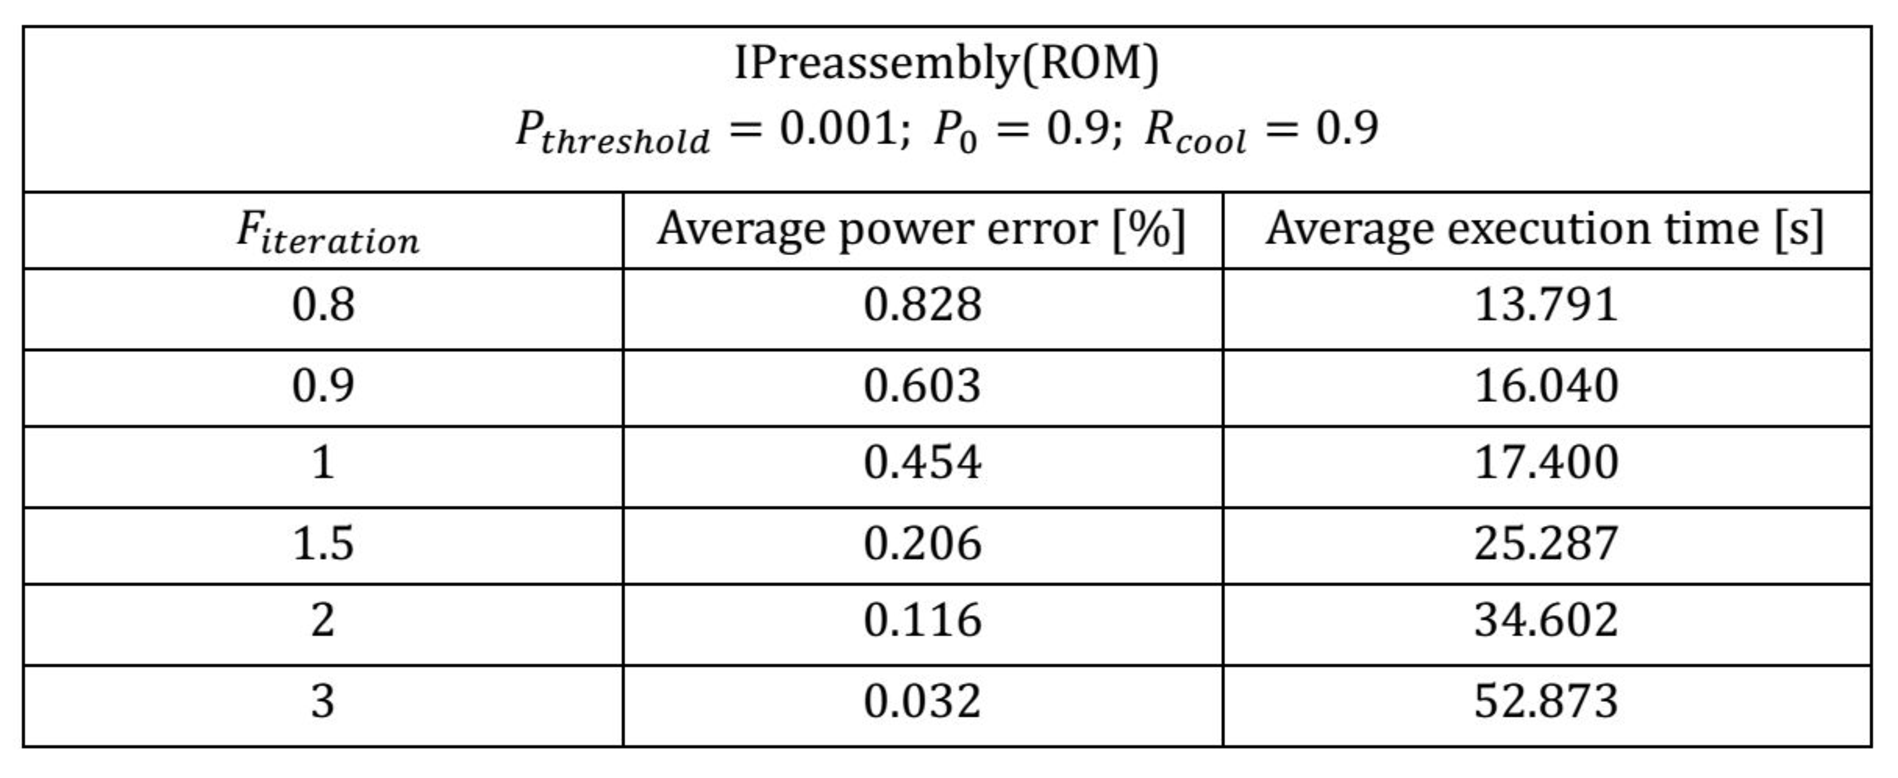
\includegraphics[width=0.7\textwidth]{EVA_FACTOR}
			\caption{FACTOR}
			\label{fig:EVA_FACTOR}
		\end{center}
	\end{figure}